% !TEX root = ../thesis.tex

In this chapter, we look at ways to implement the loopy belief propagation (LBP) algorithm on an arbitrary MRF with continuous state-spaces. We concentrate in particular on the representation of the messages and the computation of message updates in the LBP algorithm. Remember from point \ref{point:LBP} that, at iteration $n$, the messages are obtained by computing the following integral:
\eqa{
	m^{n}_{s r}(x_{r}) &=& \int \psi_{sr}(x_{s},x_{r})M^{n}_{s r}(x_{s})\dx_{s}\label{eq:mess-update-2}
}
where the pre-messages are given by 
\eqa{
	M_{r s}^{n}(x_{r}) &=& \psi_{r}(x_{r}) \prod_{u\in\partial r\backslash s} m^{n-1}_{u r}(x_{r}).
}
Ultimately, we are interested in computing the beliefs obtained by multiplying message and pre-message: $B_{r}(x_{r}) = m_{sr}(x_{r})M_{rs}(x_{r})$. There are a few main computational problems to tackle when attempting to run this algorithm in a continuous setting. First, the messages need to be represented in a tractable fashion. Second, the message updates need to be computable and the result be easily expressible in the chosen representation system. Lastly, we need to be able to sample from the resulting estimators for the beliefs. 

In this chapter, we consider the \emph{nonparametric belief propagation} (NBP) algorithm of \citet{sudderth03} and the \emph{particle belief propagation} algorithm of \citet{ihler09}. We then discuss our \emph{expectation particle belief propagation} (EPBP) algorithm \citep{lienart15} and discuss how it improves upon both. \check{jul19}

% !!!!!!!!!!!!!!!!!!!!!!!!!!!!!!!!!!!!!!!!!!!!!!!!!!!!!!!!!!!!!!!!!!!!!!!!!!!!!!!!!!!!!!!!!!!!!!!!!!
\section{Loopy Belief Propagation on Continuous State-Spaces}

%%%%%%%%%%%%%%%%%%%%%%%
\subsection{Nonparametric belief propagation}

In their paper \citet{sudderth03} suggest representing the messages in the LBP iterations as mixtures of Gaussians:
\eqa{	
	\widehat m^{\text{NBP}}_{u v}(x_{v}) &:=& \sum_{i=1}^{M} w_{v}^{i}\,\mathcal N(x_{v};\mu^{i}_{v},\Lambda_{v}). \label{eq:nbp-representation}
}
They call their algorithm \emph{nonparametric belief propagation} (NBP). In order to make computations more efficient, the authors restrict the covariance matrices to be diagonal.\add{mention this in general complaint for VI}
As indicated in the paper, the representation \eqref{eq:nbp-representation} makes sense only when the messages are finitely integrable. To guarantee this, the authors require that all potentials satisfy the following constraints:
\eqa{	
	\sup_{x_{v}} \int \psi_{uv}(x_{u},x_{v})\dx_{u} &<&\infty, \quad \text{and}\quad \int \psi_{u}(x_{u})\dx_{u} \esp<\esp \infty,\label{conditions NBP}
}
where the integrals are taken over the range of admissible values for the relevant variable. Granted these assumptions hold, the message updates are well defined and can be explicitly (and efficiently) computed. Computing the beliefs, however, requires considering the product of mixtures of $M$ terms leading to a complex representation and an explosion in computational cost. In order to alleviate this, the authors suggest an importance sampling approach targeting the beliefs and fitting mixtures of Gaussians to the resulting weighted particles. 
The computation of the message updates \eqref{eq:mess-update-2} is thereby always done over a constant number of terms.\add{proper link}\check{jul19}

\subsubsection*{Main issues}

A key weakness of this approach is that the conditions \eqref{conditions NBP} do not hold in a number of important cases (the authors aknowledge this in a footnote of their paper). 
For instance, the node potentials $\psi_{u}$ are usually proportional to likelihoods of the form $p(y_{u}\st x_{u})$ which need not be integrable in $x_{u}$. In fact, for most non-Gaussian potential, this is the case. Additionally, in imaging applications for example, the edge potential can encode a measure of similarity between pixels which also need not verify the first integrability condition as in \citet{nikolova00}.

Finally, by definition of NBP as an approximated representation with a fixed number of Gaussians, it does not offer consistent estimators of the LBP messages.\check{jul19}



%%%%%%%%%%%%%%%%%%%%
\subsection{\label{point:PBP}Particle belief propagation}

In their paper \citep{ihler09}, the authors suggest a way to overcome the shortcomings of NBP by considering importance sampling to tackle the update of the LBP messages instead of working with mixtures of Gaussians. For a chosen proposal distribution $q_{u}$ on node $u$ and a draw of $N$ particles $X_{u}^{(i)}\simiid q_{u}$, the messages are represented via an importance sampling estimator of the corresponding integral:
\eqa{		
	&\widehat m_{u v}^{\text{PBP}}(x_{v}) 
		:= \sum_{i=1}^{N}\omega^{(i)}_{uv}\psi_{uv}(X^{(i)}_{u},x_{v}), \quad\text{where}&	\label{eq:rep-PBP}\\[.3cm]
	&\omega^{(i)}_{uv} 
		\esp\!\propto\esp\! \displaystyle{\widehat M^{\text{PBP}}_{uv}(X_{u}^{(i)})\over q_{u}(X_{u}^{(i)})}, \quad\text{and}\quad
	\widehat M^{\text{PBP}}_{uv}(x_{v}) \esp\!=\esp\! \psi_{u}(x_{u}) \prod_{w\in\partial u\backslash v} \widehat m^{\text{PBP}}_{wu}(x_{u}).&\nn
}

They call their algorithm \emph{particle belief propagation} (PBP).
This algorithm has the advantage that it does not require the integrability conditions \eqref{conditions NBP} to hold. 
In terms of choosing proposals, the authors suggest two potential choices: sampling from the local potential $\psi_{u}$, or sampling from the current belief estimate on the node. 
%For the latter, the authors suggest running a short MCMC simulation. \add{explain how they build representation of beliefs}

\subsubsection{Main issue}

The weak point of the PBP algorithm is the choice of proposal distributions.  A poor choice will lead to poor estimators of the messages which, over a few iterations of the LBP algorithm, will lead to poor representation of the beliefs.

The first suggestion by the authors to sample from the local potential is only valid if $\psi_{u}$ is integrable with respect to $x_{u}$ which, as we have mentioned earlier, is not the case in general. The second suggestion implies sampling from a distribution of the form
%
\eqa{		
	\widehat B_{u}^{\text{PBP}}(x_{u}) 
		&\propto& \psi_{u}(x_{u}) \prod_{w\in\partial u} \widehat m^{\text{PBP}}_{wu}(x_{u})	\label{eq:PBP proposal}
}
%
which is a product of mixtures of $N$ components. As in nonparametric BP, naive sampling of the proposal has complexity $\mathcal O {(N^{|\partial {u}|})}$ and is thus, in general, too expensive to consider.\add{Gamma u discussed in notations?} 

Alternatively the author suggest running a short MCMC simulation targeting it which reduces the complexity to order $\mathcal O {(|\partial {u}|N^{2})}$. Indeed, each MCMC iteration requires evaluating $\widehat B_{u}^{\text{PBP}}$ point-wise which has complexity $\mathcal O {(|\partial{u}|N)}$, and we need at least $\mathcal{O}(N)$ iterations of the MCMC simulation to produce the samples. Note that it is unclear how many more iterations are necessary to get $N$ \emph{good} samples. Running a short MCMC chain (to reduce computational cost) will therefore almost certainly lead to biased samples. In the code the authors shared with us, they run $N$ parallel random walk Metropolis-Hastings (RWMH) for a fixed number of steps. \add{there should probably be an additional comment on this in discussion}


% !!!!!!!!!!!!!!!!!!!!!
\section{Expectation Particle Belief Propagation}
As for the PBP algorithm, we consider importance sampling to build particle representations of the messages. In our method, however, we consider a \emph{sequence} of proposal distributions at each node from which one can cheaply sample particles at a given iteration of the LBP algorithm. 

The novelty of the approach is to propose a principled and automated way of designing a sequence of proposals in a tractable exponential family using the expectation propagation (EP) algorithm. The resulting method, which we call \emph{Expectation Particle Belief Propagation} (EPBP), does not suffer from the restrictive integrability conditions of the NBP algorithm and sampling is done exactly unlike the PBP algorithm which implies that we obtain consistent estimators of the LBP messages.

Further, the development of our method also formally shows that considering proposals close to the beliefs, as suggested by \cite{ihler09}, is a good idea.  Our core observation is that since sampling from a proposal of the form \eqref{eq:PBP proposal} using MCMC simulation is very expensive, we should consider using a more tractable proposal distribution instead. However it is important that the proposal distribution is constructed adaptively, taking into account evidence collected through the message passing itself. We propose to achieve this by using proposal distributions lying in a tractable exponential family, and adapted using EP.

%%%%%%%%%%%%%%%%
\subsection{Proposal selection for PBP}
In this point we discuss the ideal choice of proposal distributions when considering the PBP algorithm. We consider two connected nodes $s$ and $t$ at a a given iteration and assume we have already constructed particle based representations of all incoming messages into both $s$ and $t$ apart from the messages from $s$ to $t$ and from $t$ to $s$. 
We therefore have both pre-messages $\widehat M_{st}$ and $\widehat M_{ts}$ of the form:
%
\eqa{
	\widehat M_{st}(x_{s}) &\propto& \psi_{s}(x_{s}) \prod_{r\in \partial s \backslash t} \widehat m_{rs}(x_{s}).
}
%
This is illustrated at figure \ref{representation-edge-pbp}. 

\begin{figure}[!h]
\center
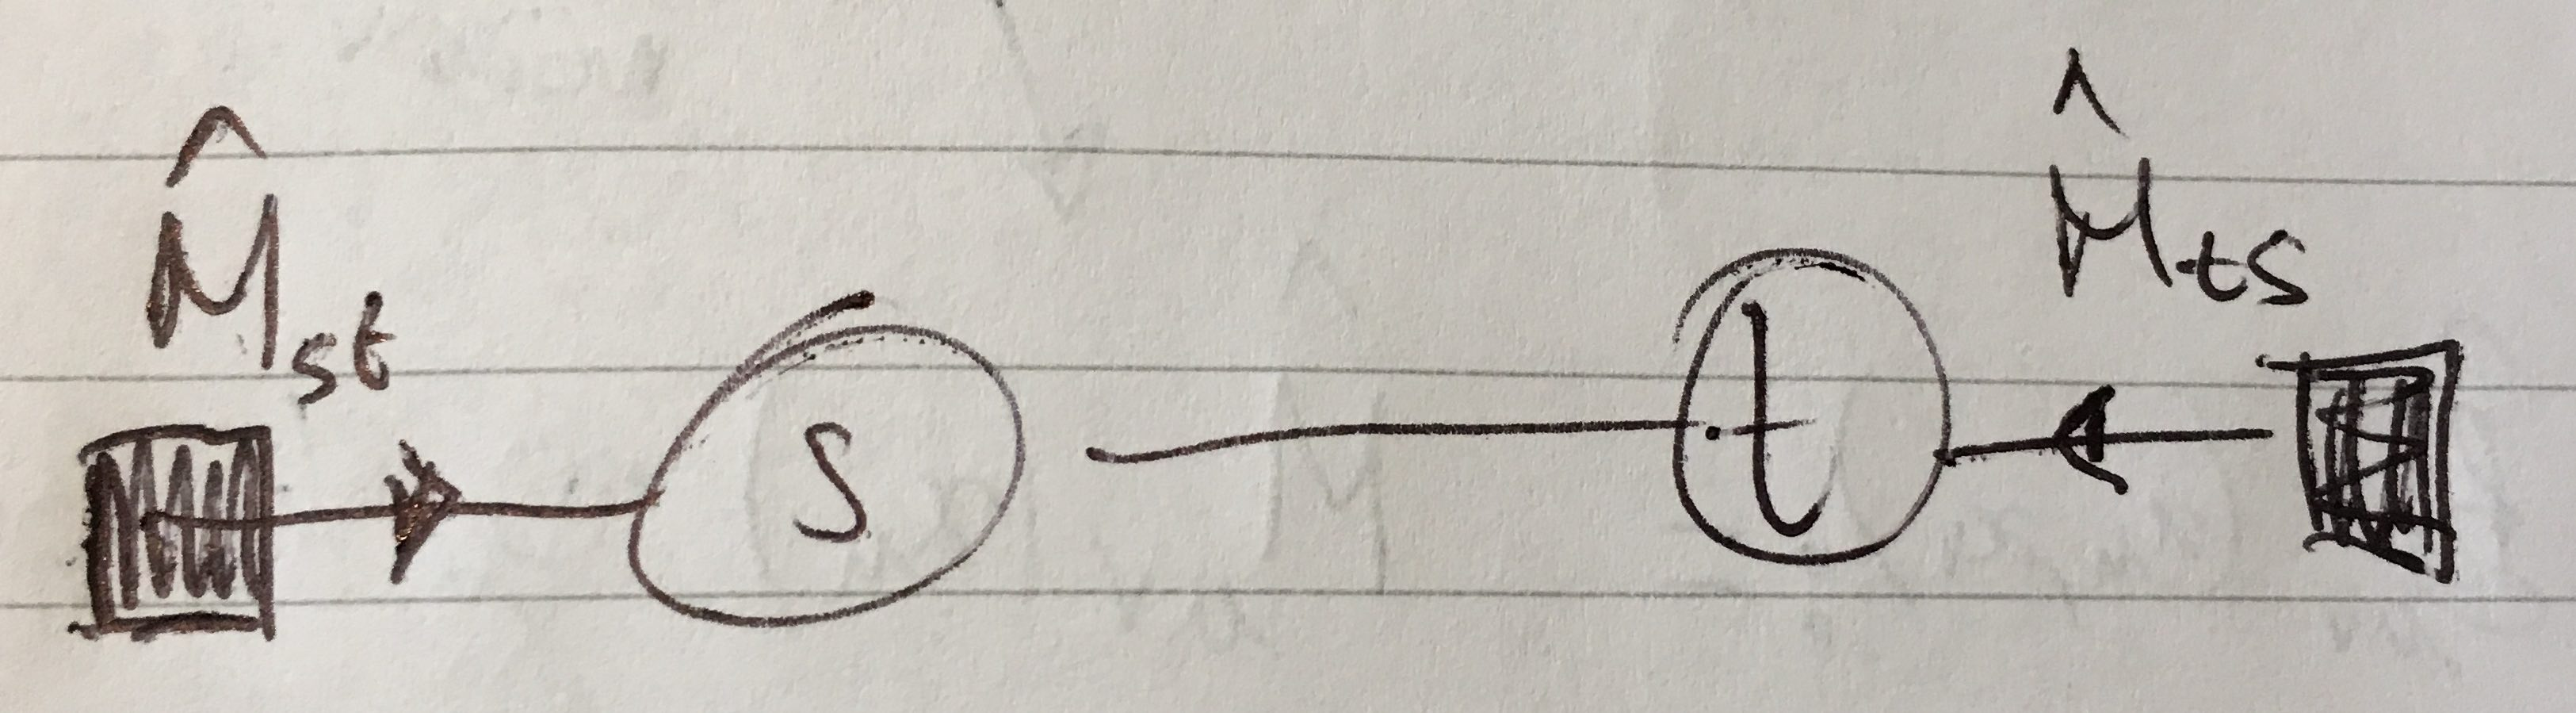
\includegraphics[width=.7\textwidth]{figures/draft/schema_pbpsel}
\caption{\label{representation-edge-pbp}}
\end{figure}

We would like to define $q_{s}$ and $q_{t}$ in a joint manner in such a way that all objects remain consistent with the LBP iterations. For that reason, we consider the joint belief $ B_{st}$ on $s$ and $t$ given the approximation to the pre-messages:
%
\eqa{	
	 B_{st}(x_{s},x_{t}) &\propto& \widehat M_{st}(x_{s}) \psi_{st}(x_{s},x_{t})\widehat M_{ts}(x_{t}).
}
%
The marginals of the joint belief are of the form
%
\eqa{
	B_{st}(x_{s}) &\propto& \widehat M_{ts}(x_{s}) \int \psi_{st}(x_{s},x_{t}) \widehat M_{ts}(x_{t})\dx_{t}\nn\\
	&\propto & \widehat M_{st}(x_{s}) m_{ts}(x_{s}),
}
%
where $m_{ts}$ is the true LBP message given the pre-message approximation $\widehat M_{ts}$.
Following our point about defining $q_{s}$ and $q_{t}$ in a joint manner, let us consider $q_{s}q_{t}$ as a proposal for the joint belief $ B_{st}$.
We can then define an empirical distribution for it:
%
\eqa{
	\widehat{B}_{st}(x_{s},x_{t}) &\propto& \sum_{i,j=1}^{N} {\widehat M_{st}(X_{s}^{(i)})\psi_{st}(X_{s}^{(i)},X_{t}^{(j)})\widehat M_{ts}(X_{t}^{(j)}) \over q_{s}(X_{s}^{(i)})q_{t}(X_{t}^{(j)})} \delta_{(X_{s}^{(i)},X_{t}^{(j)})}(x_{s},x_{t}). \label{eq:pbp-particle-joint-belief}
}
%
Marginalising this approximation over $x_{t}$ leads to
%
\eqa{
	\widehat{B}_{st}(x_{s}) &\propto& \sum_{i=1}^{N} {\widehat M_{st}(X_{s}^{(i)}) \widehat { m}_{ts}(X_{s}^{(i)}) \over q_{s}(X_{s}^{(i)})} \delta_{X_{s}^{(i)}}(x_{s}). \label{eq:pbb-particle-joint-belief-marg}
}
%
where $\widehat{m}_{ts}$ is the importance sampling estimator for $\overline m_{ts}$ using $q_{t}$ as proposal. Of course, marginalising \eqref{eq:pbp-particle-joint-belief} over $x_{s}$ leads to an expression analogous to \eqref{eq:pbb-particle-joint-belief-marg}. Focusing on node $s$, the expression \eqref{eq:pbb-particle-joint-belief-marg} indicate that the proposals should be given by
%
\eqa{
	q_{s}(x_{s}) &\propto& \widehat{M}_{st}(x_{s}) \widehat{m}_{ts}(x_{s}) \esp = \esp \psi_{s}(x_{s}) \prod_{r\in\partial s} \widehat{m}_{rs}(x_{s})
	}
where all $\widehat m_{rs}$ are IS estimators built using the corresponding (most recent) $q_{r}$ as a proposal. Further, this shows that the proposals on nodes should correspond to the most recent approximation of the belief at that node which aligns with the suggestion in \citet{ihler09}.

%%%%%%%%%%%%%%%%
\subsection{The EPBP algorithm}
As we showed in point \ref{point:PBP}, it is computationally expensive to use the particle approximated node belief as the proposal distribution. 
Our idea is to consider an approximation $q_{u}$ drawn from a tractable exponential family $\mathcal F_{\phi}$ with a structure matching that of the belief:
%
\eqa{ 
	q_u(x_u) &\propto& \eta_{\circ u}(x_u) \prod_{w\in\Gamma_u} \eta_{wu}(x_u).
}
%
In the experiments we used a Gaussian family but we are not limited to this (in theory).
Using the framework of expectation propagation (EP) that we discussed in point \ref{point:EP}, we can iteratively find good exponential family approximations.\\

Following the EP framework, for each $w\in\Gamma_u$, to update the $\eta_{wu}$, we form the \emph{cavity} $q^{\backslash w}_{u}=q_{u}/\eta_{wu}$ and the corresponding \emph{tilted distribution} proportional to $\widehat m_{wu} q_{u}^{\backslash w}$.  The updated distribution is then the projection of the tilted distribution onto the exponential family manifold:
\eqa{ q_{u} &\leftarrow& \mathcal P_{\phi}[\widehat m_{wu}q_{u}^{\backslash w}],}	
where $\mathcal P_{\phi}$ is the projection operator introduced in \hyperref[sec:projop]{point~\ref*{sec:projop}}. Consequently, the factor $\eta_{wu}$ is updated: $\eta_{wu} \leftarrow  q_{u}/ q_{u}^{\backslash w}$.

%%%%%%%%%%%%%%%%%%%%%%
\subsection{Alternative projection methods}

%%%%%%%%%%%%%%%%%
\subsection{EPBP for smoothing}

%%%%%%%%%%%
\section{Experiments}

\section{Discussion}

\todofr{
\begin{itemize}
\item watch out to not stress consistency for subquad algo (consistency probably incorrect anyway as per conversation with Naesseth)
\item discuss existing, PBP, NBP etc. explain that NBP probably good for most cases (?) a little bit like KF for HMM.
\end{itemize}
}